\documentclass[journal,12pt,twocolumn]{IEEEtran}

\usepackage{setspace}
\usepackage{gensymb}

\singlespacing


\usepackage[cmex10]{amsmath}

\usepackage{amsthm}

\usepackage{mathrsfs}
\usepackage{txfonts}
\usepackage{stfloats}
\usepackage{bm}
\usepackage{cite}
\usepackage{cases}
\usepackage{subfig}

\usepackage{longtable}
\usepackage{multirow}

\usepackage{enumitem}
\usepackage{mathtools}
\usepackage{steinmetz}
\usepackage{tikz}
\usepackage{circuitikz}
\usepackage{verbatim}
\usepackage{tfrupee}
\usepackage[breaklinks=true]{hyperref}

\usepackage{tkz-euclide}

\usetikzlibrary{calc,math}
\usepackage{listings}
    \usepackage{color}                                            %%
    \usepackage{array}                                            %%
    \usepackage{longtable}                                        %%
    \usepackage{calc}                                             %%
    \usepackage{multirow}                                         %%
    \usepackage{hhline}                                           %%
    \usepackage{ifthen}                                           %%
    \usepackage{lscape}     
\usepackage{multicol}
\usepackage{chngcntr}

\DeclareMathOperator*{\Res}{Res}

\renewcommand\thesection{\arabic{section}}
\renewcommand\thesubsection{\thesection.\arabic{subsection}}
\renewcommand\thesubsubsection{\thesubsection.\arabic{subsubsection}}

\renewcommand\thesectiondis{\arabic{section}}
\renewcommand\thesubsectiondis{\thesectiondis.\arabic{subsection}}
\renewcommand\thesubsubsectiondis{\thesubsectiondis.\arabic{subsubsection}}


\hyphenation{op-tical net-works semi-conduc-tor}
\def\inputGnumericTable{}                                 %%

\lstset{
%language=C,
frame=single, 
breaklines=true,
columns=fullflexible
}
\begin{document}


\newtheorem{theorem}{Theorem}[section]
\newtheorem{problem}{Problem}
\newtheorem{proposition}{Proposition}[section]
\newtheorem{lemma}{Lemma}[section]
\newtheorem{corollary}[theorem]{Corollary}
\newtheorem{example}{Example}[section]
\newtheorem{definition}[problem]{Definition}

\newcommand{\BEQA}{\begin{eqnarray}}
\newcommand{\EEQA}{\end{eqnarray}}
\newcommand{\define}{\stackrel{\triangle}{=}}
\bibliographystyle{IEEEtran}
\providecommand{\mbf}{\mathbf}
\providecommand{\pr}[1]{\ensuremath{\Pr\left(#1\right)}}
\providecommand{\qfunc}[1]{\ensuremath{Q\left(#1\right)}}
\providecommand{\sbrak}[1]{\ensuremath{{}\left[#1\right]}}
\providecommand{\lsbrak}[1]{\ensuremath{{}\left[#1\right.}}
\providecommand{\rsbrak}[1]{\ensuremath{{}\left.#1\right]}}
\providecommand{\brak}[1]{\ensuremath{\left(#1\right)}}
\providecommand{\lbrak}[1]{\ensuremath{\left(#1\right.}}
\providecommand{\rbrak}[1]{\ensuremath{\left.#1\right)}}
\providecommand{\cbrak}[1]{\ensuremath{\left\{#1\right\}}}
\providecommand{\lcbrak}[1]{\ensuremath{\left\{#1\right.}}
\providecommand{\rcbrak}[1]{\ensuremath{\left.#1\right\}}}
\theoremstyle{remark}
\newtheorem{rem}{Remark}
\newcommand{\sgn}{\mathop{\mathrm{sgn}}}
\providecommand{\abs}[1]{\left\vert#1\right\vert}
\providecommand{\res}[1]{\Res\displaylimits_{#1}} 
\providecommand{\norm}[1]{\left\lVert#1\right\rVert}
%\providecommand{\norm}[1]{\lVert#1\rVert}
\providecommand{\mtx}[1]{\mathbf{#1}}
\providecommand{\mean}[1]{E\left[ #1 \right]}
\providecommand{\fourier}{\overset{\mathcal{F}}{ \rightleftharpoons}}
%\providecommand{\hilbert}{\overset{\mathcal{H}}{ \rightleftharpoons}}
\providecommand{\system}{\overset{\mathcal{H}}{ \longleftrightarrow}}
	%\newcommand{\solution}[2]{\textbf{Solution:}{#1}}
\newcommand{\solution}{\noindent \textbf{Solution: }}
\newcommand{\cosec}{\,\text{cosec}\,}
\providecommand{\dec}[2]{\ensuremath{\overset{#1}{\underset{#2}{\gtrless}}}}
\newcommand{\myvec}[1]{\ensuremath{\begin{pmatrix}#1\end{pmatrix}}}
\newcommand{\mydet}[1]{\ensuremath{\begin{vmatrix}#1\end{vmatrix}}}
\numberwithin{equation}{subsection}
\makeatletter
\@addtoreset{figure}{problem}
\makeatother
\let\StandardTheFigure\thefigure
\let\vec\mathbf
\renewcommand{\thefigure}{\theproblem}
\def\putbox#1#2#3{\makebox[0in][l]{\makebox[#1][l]{}\raisebox{\baselineskip}[0in][0in]{\raisebox{#2}[0in][0in]{#3}}}}
     \def\rightbox#1{\makebox[0in][r]{#1}}
     \def\centbox#1{\makebox[0in]{#1}}
     \def\topbox#1{\raisebox{-\baselineskip}[0in][0in]{#1}}
     \def\midbox#1{\raisebox{-0.5\baselineskip}[0in][0in]{#1}}
\vspace{3cm}
\title{EE5609 Assignment 5}
\author{Abhishek Thakur}
\maketitle
\newpage
\bigskip
\renewcommand{\thefigure}{\theenumi}
\renewcommand{\thetable}{\theenumi}
\begin{abstract}
This document contains the solution of geometry through linear algebra.
\end{abstract}
Download latex and python codes from 
\begin{lstlisting}
https://github.com/abhishekt711/EE5609/tree/master/Assignment_5
\end{lstlisting}
%
\section{Problem}
Prove that the following equations represent two straight lines, find also their point of intersection and the angle between them.\\
$6y^2-xy-x^2+30y+36=0$.
\section{Explanation}
The given equation can be written as:
\begin{align}
-x^2-xy+6y^2+30y+36=0 \label{eq1}
\end{align}
\mydet{\vec{V}&\vec{u}\\\vec{u}^T&f} of \eqref{eq1} becomes
\begin{align}
    \mydet{-1&-\frac{1}{2}&0\\\frac{-1}{2}&6&15\\0&15&36}=0\label{eq02}
\end{align}
Expanding equation \eqref{eq02}, we get zero.\\
Hence given equation represents a pair of straight lines.

The general equation second degree is given by
\begin{equation}\label{eq5}
	ax^2 + 2bxy + cy^2 + 2dx + 2ey + f = 0
\end{equation}
Let $(\alpha,\beta)$ be their point of intersection, then
\begin{equation}\label{eq6}
	\myvec{ a & h\\ h & b}\myvec{\alpha \\ \beta} = \myvec{-d \\ -e}
\end{equation}
Under \textit{Affine transformation},
\begin{align}
	\vec{x} &= \vec{M}\vec{y} + c\\
	\myvec{x \\ y} &= \myvec{1 & 0 \\ 0 & 1} \myvec{X \\ Y} + \myvec{\alpha \\ \beta}\\
	\label{eq7}\myvec{x \\ y} &= \myvec{X+\alpha \\ Y+\beta}
\end{align}
\eqref{eq5} under transformation \eqref{eq7} will become,
\begin{equation}\label{eq8}
	aX^2 + 2bXY + cY^2 = 0
\end{equation}
\begin{equation}\label{eq9}
	\myvec{X & Y} \myvec{a & h \\ h & b} \myvec{X \\ Y} = 0
\end{equation}
%\begin{equation}\label{eq10}
%	\vec{X}^T\vec{V}\vec{X} = 0
%\end{equation}
\begin{equation}\label{eq11}
	\myvec{X & Y} \myvec{u_1 & v_1 \\ u_2 & v_2} \myvec{\lambda_1 & 0\\ 0 & \lambda_2} \myvec{u_1 & u_2 \\ v_1 & v_2} \myvec{X \\ Y} = 0
\end{equation}
\begin{equation}
	\myvec{X^\prime & Y^\prime}  \myvec{\lambda_1 & 0\\ 0 & \lambda_2} \myvec{X^\prime \\ Y^\prime} = 0
\end{equation}
\begin{equation}\label{eq12}
	\text{where } X^\prime = Xu_1 + Yu_2 \text{ and } Y^\prime = Xv_1 + Yv_2
\end{equation}
\begin{equation}\label{eq13}
	\implies \lambda_1 (X^\prime)^2 + \lambda_2 (Y^\prime)^2 = 0
\end{equation}
\eqref{eq13} is called \textit{Spectral decomposition} of matrix
\begin{align}
	\implies X^\prime &= \pm \sqrt{-\frac{\lambda_2}{\lambda_1}}Y^\prime\\	
	u_1X + u_2Y &= \pm \sqrt{-\frac{\lambda_2}{\lambda_1}}(v_1X + v_2Y)\\
	\label{eq14}u_1(x-\alpha) + u_2(y-\beta) &= \pm \sqrt{-\frac{\lambda_2}{\lambda_1}}(v_1(x-\alpha) + v_2(y-\beta))
\end{align}

Given equation is
\begin{align}
	-x^2-xy+6y^2+30y+36=0
\end{align}
Substituting in \eqref{eq6}
\begin{align}
	\label{eq16}\myvec{ -1 & \frac{-1}{2}\\\frac{-1}{2} & 6}\myvec{\alpha \\ \beta} = \myvec{0 \\ -15} \\
	\label{eq17}\implies \myvec{\alpha \\ \beta} = \myvec{\frac{30}{23} \\ \frac{-60}{23}}
\end{align}
\begin{equation}
	\text{From \textit{Spectral theorem, }}\vec{V} = \vec{P}\vec{D}\vec{P}^T
\end{equation}
\begin{align}
	\label{eq18}\vec{V} &= \myvec{ -1 & \frac{-1}{2}\\\frac{-1}{2} & 6}
\end{align}
P and D are found using python code from
\begin{lstlisting}
codes/diagonalize1.py
\end{lstlisting}
Substituting and simplifying in \ref{eq14}.
\begin{align}
	\label{eq22}-x + 2y + 6 = 0 \text{ and } x + 3y + 6 = 0\\
	\implies (-x + 2y + 6)(x + 3y + 6) = 0
\end{align}

\text{Hence, the intersection point is}
\myvec{\frac{6}{5}\\-\frac{12}{5}}\\
Verified using python code from
\begin{lstlisting}
codes/Assignment_5.py
\end{lstlisting}
Also, from the given equation:
\begin{align}
-x^2-xy+6y^2+30y+36=0 \label{eq1}
\end{align}
Slopes of the individual lines are roots of equation 
\begin{align}
    cm^2+2bm+a=0\\
    \implies 6m^2-m-1=0\\
    \text{Solving, }m=\frac{1}{2},-\frac{1}{3}
\end{align}
The normal vectors of the lines then become
\begin{align}
    \vec{n_1}=\myvec{-1\\2}\\
    \vec{n_2}=\myvec{1\\3}
\end{align}
Equations of the lines can therefore be written as
\begin{align}
  \myvec{-1&2}\vec{x}=c_1\\
   \myvec{1&3}\vec{x}=c_2\\
  \implies \left[\myvec{-1&2}\vec{x}-c_1\right]\left[\myvec{1&3}\vec{x}-c_2\right]
\end{align}
represents the equation specified in \eqref{eq1}\\
Comparing the equations, we have
\begin{align}
    \myvec{-1&1\\2&3}\myvec{c_2\\c_1}=\myvec{0\\-30}\\
 \end{align}
 Row reducing the augmented matrix
 \begin{align}
    \myvec{-1&1&0\\2&3&-30}\xleftrightarrow[]{R_2\leftarrow R_2+2\times R_1}
    \myvec{-1&1&0\\0&5&-30}\\
    \xleftrightarrow[]{R_2\leftarrow R_1- R_2\times \frac{1}{5}}
    \myvec{-1&0&6\\0&5&-30}\\
    \xleftrightarrow[]{R_1\leftarrow -1\times R_1  , R_2\leftarrow \frac{1}{5}\times R_2}
    \myvec{1&0&-6\\0&1&-6}\\
    \implies c_1=-6 \text{ and }c_2=-6
\end{align}
The individual line equations therefore become
\begin{align}
    \myvec{-1&2}\vec{x}=-6\label{eq3} ,\\\myvec{1&3}\vec{x}=-6\label{eq4}
\end{align}
Note that the convolution of the normal vectors, should satisfy the below condition
\begin{align}
    \myvec{-1\\2}*\myvec{1\\3}=\myvec{a\\2b\\c}\label{eq5}
\end{align}
The LHS part of \eqref{eq5} can be rewritten using toeplitz matrix as
\begin{align}
    \myvec{-1&0\\2&-1\\0&2}\myvec{1\\3}=\myvec{-1\\-1\\6}=\myvec{a\\2b\\c}
\end{align}
The augmented matrix for the set of equations represented in \eqref{eq3}, \eqref{eq4} is
\begin{align}
\myvec{-1&2&-6\\1&3&-6}
\end{align}
Row reducing the matrix
\begin{align}
 \myvec{-1&2&-6\\1&3&-6}\xleftrightarrow[]{R_2\leftarrow R_2+R_1}\myvec{-1&2&-6\\0&5&-12}\\
 \xleftrightarrow[]{R_1\leftarrow R_1-\frac{2}{5}\times R_2}\myvec{-1&0&-\frac{6}{5}\\0&5&-12}\\
 \xleftrightarrow[]{R_1\leftarrow -1\times R_1  , R_2\leftarrow \frac{1}{5}\times R_2}\myvec{1&0&\frac{6}{5}\\0&1&-\frac{12}{5}}\\
\text{Hence, the intersection point is}
\myvec{\frac{6}{5}\\-\frac{12}{5}}
\end{align}



Angle between two lines $\theta$ can be given by
\begin{align}
\cos \theta = \frac{\vec{n_1}^T\vec{n_2}}{\norm{\vec{n_1}}\norm{\vec{n_2}}}
\end{align}
%From \eqref{eq:solutions/13/3/3}, \eqref{eq:solutions/13/3/4},
\begin{align}
&\cos \theta=\frac{\myvec{-1&2}\myvec{1\\3}}{\sqrt{(-1)^2 +(2)^2} \times \sqrt{1 +(3)^2}}=\frac{1}{\sqrt{2}}\\
&\implies \theta = 45\degree
\end{align}
\begin{figure}[!ht]
\centering
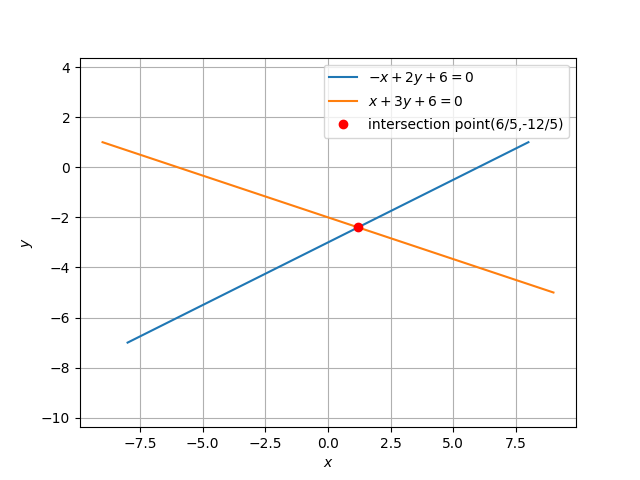
\includegraphics[width=\columnwidth]{Figure_1.png}
\caption{plot showing intersection of lines.}
\label{Fig_1}
\end{figure}

\end{document}